\RequirePackage[l2tabu, orthodox]{nag}
\documentclass{article}
\usepackage[letterpaper]{geometry}
\usepackage{siunitx}
\usepackage{multicol}
\usepackage{graphicx}
\usepackage{float}
\usepackage{minted}
\usepackage{booktabs}
\usepackage{subcaption}
\usepackage{hyperref}
\usepackage{fontspec}
\usepackage{multirow}
\usepackage{listings}
\usepackage{xcolor}
\usepackage{pgfplots}
\usepackage{pgfplotstable}
\usepackage{caption}
\usepackage{subcaption}
\usepackage{pdfpages}

\setmainfont{Noto Serif}
\setmonofont{Source Code Pro}

\usemintedstyle{xcode}
\setminted{fontsize=\footnotesize, linenos=true}

\begin{document}

\begin{titlepage}
    \begin{center}
        \vspace*{1cm}

        \textbf{\Large{Lab 3}}

        \vspace{0.5cm}

        \LARGE{Communication via SPI}
        \vspace{1.5cm}

        Michael Kwok

        \vfill
        \Large{ECE 315 Lab H41\\
            Department of Electrical and Computer Engineering\\
            University of Alberta\\
            1 April 2021}
    \end{center}
\end{titlepage}
\newpage
\tableofcontents
\thispagestyle{empty}
\newpage
\section{Abstract}
The Zybo Z7 is a digital logic and embedded software development platform by Digilent, containing a Zybo 7000 System on a Chip (SoC) that has both a digital logic fabric (Xilinx 7-series FPGA) and a hard processor (ARM Cortex-A9). For this lab, we will be making use of UART and SPI for communication between tasks and peripherals.\@

In the first part of the lab, we updated the task that is acting as a slave peripheral to count bytes sent to it, and print out the statistics for all tasks. In the 2nd part of the lab, we write code to generate artificial load on the CPU to calculate how much work can be done on the CPU.\@

All code for this lab has been attached in the Appendix.

\section{Design}

This lab is mostly an echo program with printing statistics. Four tasks were used in total, each performing a specific role. A diagram representing the architecture is shown in figure~\ref{fig1:arch}. As mentioned in the appendix, a core component of this lab is the use of SPI, with the single board having both an SPI master and SPI slave.

The role of UART in this lab is solely for user interface communication. It's used for the user to input selections on the main menu on what action to do, and for showing the response of the SPI communications. The program is able to run in loopback mode, where SPI is not used, or IPC via queues are not used either, which is useful for testing if the system runs as expected before attempting to set up SPI communications.

\begin{figure}
    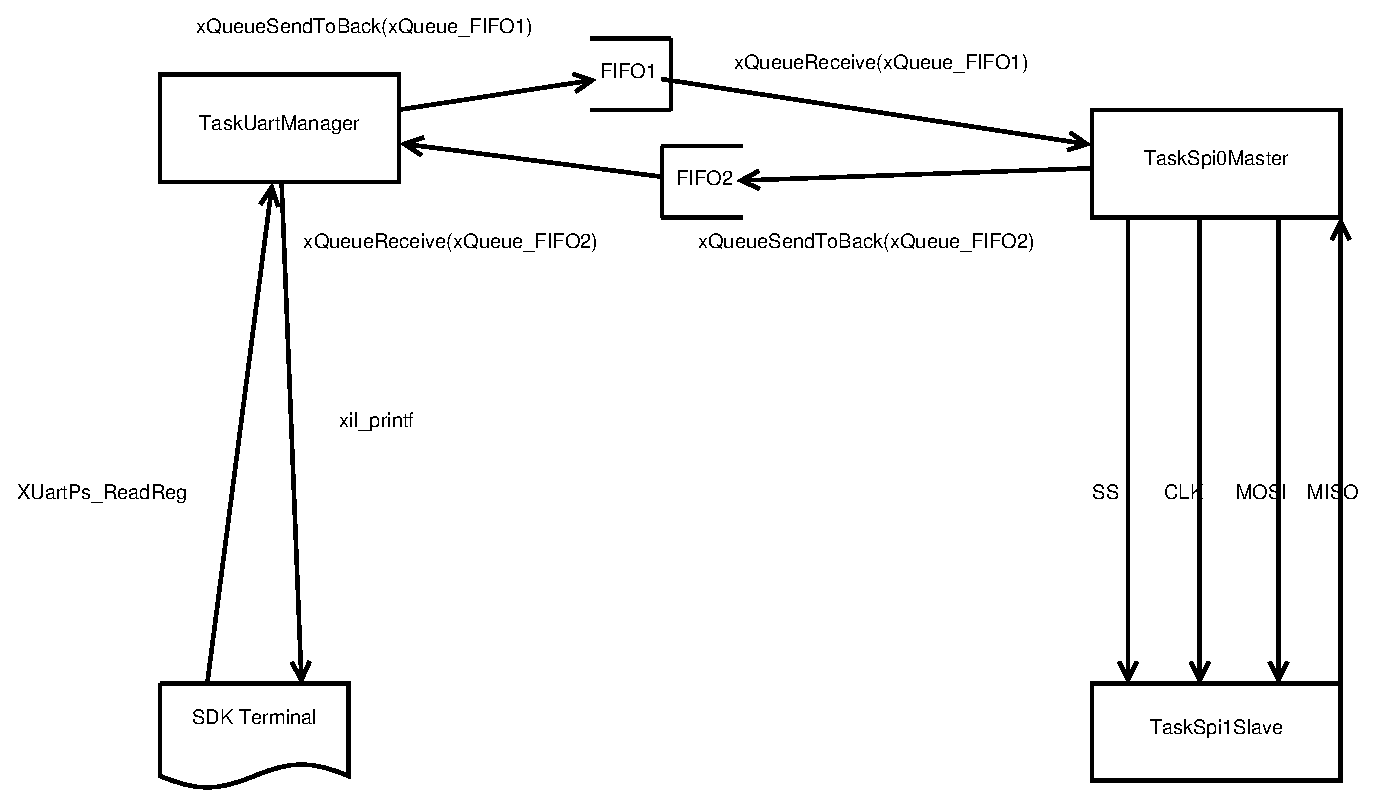
\includegraphics[width=\linewidth]{Diagram1.eps}
    \caption{Architecture of the lab}
    \label{fig1:arch}
\end{figure}

\subsection{Part 1}
The first part of the lab specifically handles the use of SPI.\@ For this, the slave task has to be modified to be able to detect the sequence \verb|\r#\r|, referred to as the termination sequence, before pushing out statistics about the communication so far via SPI back to the master. The statistics sent are: bytes processed, and task workload information.

A simple ring buffer-like data structure is used as memory to ensure that the desired sequence as been entered. Once this sequence is input, the task begins to generate the string to send via SPI from the slave to the master.\@ An example of the string generated by the slave task is shown in listing~\ref{list1:example}. The strings are formed via the use of \verb|snprintf| and a format string for the first sentence, then by calling the FreeRTOS function \verb|vTaskGetRunTimeStats| for the requested statistics.

SPI is a full duplex serial interface created by Motorola in the 1980s. SPI requires a master-slave architecture, where one peripheral is designated as the master, telling the slave when to communicate, and the slave simply responding to master requests. Being full duplex, it allows communication at the same time both ways. However, the way this is done is different to how most modern protocols do it. For SPI, the inputs and outputs are stored in a shift register, so for every read, it has to be replenished with another byte to avoid FIFO underflows.

This last fact leads to the main issue of the lab, as we are required to send more from the slave than we receive in data from the master peripheral. The solution for this is to send a pre-determined control character that is simply an ASCII character that is rarely used, which in this project was chosen to be \verb|0x07| or the ASCII bell control character. After the string to be sent has been determined, a global with the expected size of transmission is set. This allows the other tasks to know that it should be sending control characters to the slave to ensure the shift registers stay at the required levels.

The task chosen to do this was Task 1 or \verb|TaskUartManager|. It was chosen as the high default priority means that priority management could be circumvented, reducing the difficulty of the task. The main task sends a single byte with the ASCII bell character to \verb|FIFO1| which the master then takes to send to the slave. The slave upon receiving the bell character will send a byte of the statistics requested, which is then pushed into \verb|FIFO2| when the master task receives it. This is repeated until all the bytes have been sent, and the tasks will return to normal operation again. To ensure that this process runs without user intervention, it's outside the main loop that checks for new UART input, instead checking independently.
\begin{lstlisting}[caption={Example of output after termination sequence}, label={list1:example}]
    The number of characters received over SPI: 3.
    TASK3	4460		20%
    TASK2	0		<1%
    TASK4	0		<1%
    IDLE	16996		79%
    TASK1	24		<1%
    Tmr Svc	0		<1%
\end{lstlisting}

\subsection{Part 2}
For the second part of the lab, it's simply the addition for a new menu item in the UART task, which is used to control task 4 in the program. This task runs an artificial load on the CPU of the board, which is XORing a value over and over again with a certain number of iterations. It was used to count the amount of cycles required to get a certain load percentage on the system. The results collected are in table~\ref{tab:tabl} and graphed in figure~\ref{graph:grap}.

A block design screenshot is attached at the appendix.

\begin{figure}
    \centering
    \begin{subfigure}[b]{0.4\textwidth}
        \begin{tabular}{cc}
            \toprule
            Iterations & Idle Percentage \\
            \midrule
            10000      & 80\%            \\
            15000      & 86\%            \\
            20000      & 30\%            \\
            25000      & 19\%            \\
            30000      & 13\%            \\
            35000      & 8\%             \\
            40000      & 11\%            \\
            45000      & 11\%            \\
            50000      & 20\%            \\
            75000      & 14\%            \\
            100000     & 25\%            \\
            200000     & 18\%            \\
            300000     & 16\%            \\
            400000     & 17\%            \\
            500000     & 15\%            \\
            \bottomrule
        \end{tabular}
        \caption{Table of Experimental Results}
        \label{tab:tabl}
    \end{subfigure}
    \begin{subfigure}[b]{0.4\textwidth}
        \begin{tikzpicture}
            \begin{axis}[
                    title={Iterations vs Idle Percentage},
                    xlabel={Iterations},
                    ylabel={Idle Percentage},
                    xmin=9000, xmax=200000,
                    ymin=0, ymax=100,
                    legend pos=north west,
                    ymajorgrids=true,
                    grid style=dashed,
                ]
                \pgfplotstableread{data.dat}\mydata

                \addplot[color=blue,mark=square,] table{\mydata};
            \end{axis}
        \end{tikzpicture}
        \caption{Graph of Experimental Results}
        \label{graph:grap}
    \end{subfigure}
    \caption{Experimental Results}
\end{figure}

\section{Conclusion}
SPI is a powerful communication interface, as it's simple to implement and use, while also being extremely flexible. While it's not very fast, it's fast enough for most purposes, especially in the embedded space. Using an RTOS also allows the developer to mix different forms of communication interfaces to achieve a singular goal, which is useful as some things might be easier in one interface than another.

The manual tuning of values to calculate CPU usage was unsuccessful however. This could be due to hardware issues such as overheating or due to some bug in the other code that affected the pre-emptive multitasking scheduler of the RTOS used.
\newpage
\appendix
\section{Code}
\inputminted{C}{SPI_main.c}
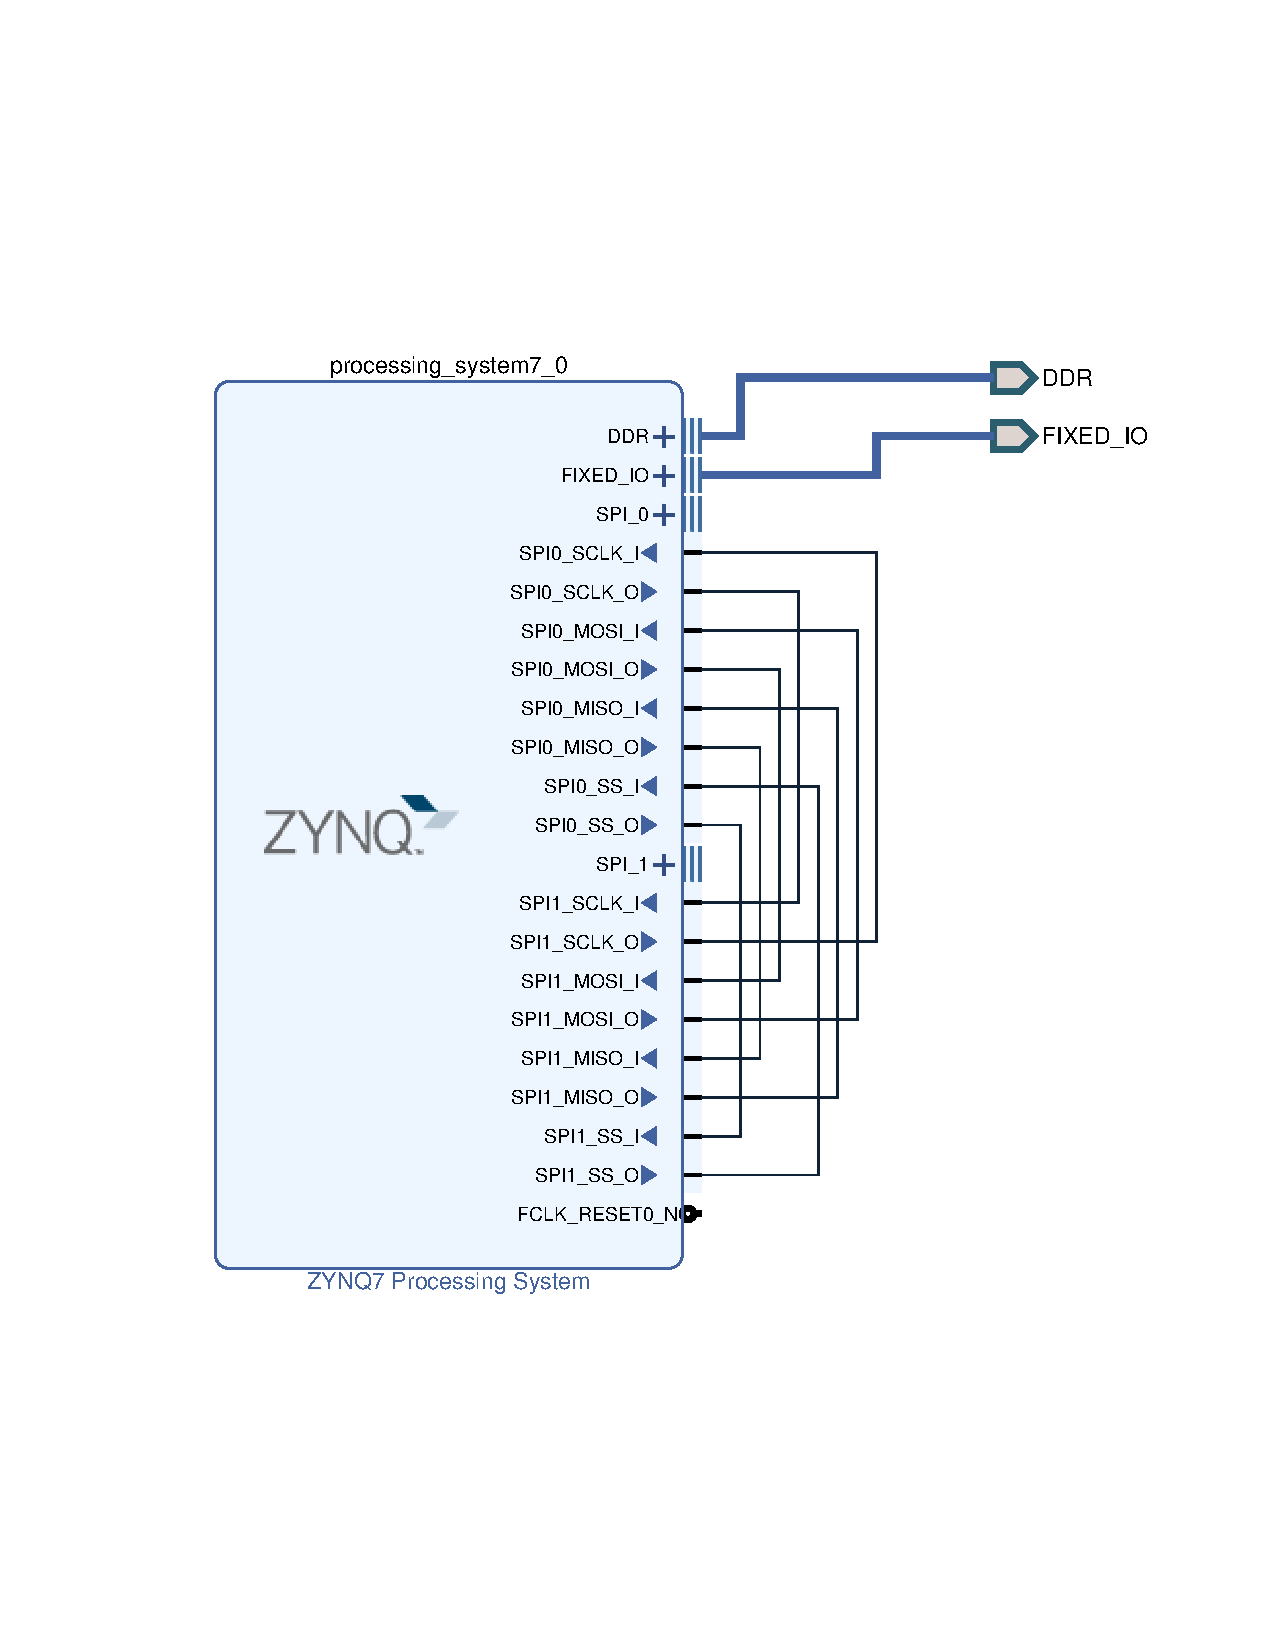
\includepdf[pages=-]{design_1.pdf}
\end{document}
